% Options for packages loaded elsewhere
\PassOptionsToPackage{unicode}{hyperref}
\PassOptionsToPackage{hyphens}{url}
%
\documentclass[
  ignorenonframetext,
]{beamer}
\usepackage{pgfpages}
\setbeamertemplate{caption}[numbered]
\setbeamertemplate{caption label separator}{: }
\setbeamercolor{caption name}{fg=normal text.fg}
\beamertemplatenavigationsymbolsempty
% Prevent slide breaks in the middle of a paragraph
\widowpenalties 1 10000
\raggedbottom
\setbeamertemplate{part page}{
  \centering
  \begin{beamercolorbox}[sep=16pt,center]{part title}
    \usebeamerfont{part title}\insertpart\par
  \end{beamercolorbox}
}
\setbeamertemplate{section page}{
  \centering
  \begin{beamercolorbox}[sep=12pt,center]{part title}
    \usebeamerfont{section title}\insertsection\par
  \end{beamercolorbox}
}
\setbeamertemplate{subsection page}{
  \centering
  \begin{beamercolorbox}[sep=8pt,center]{part title}
    \usebeamerfont{subsection title}\insertsubsection\par
  \end{beamercolorbox}
}
\AtBeginPart{
  \frame{\partpage}
}
\AtBeginSection{
  \ifbibliography
  \else
    \frame{\sectionpage}
  \fi
}
\AtBeginSubsection{
  \frame{\subsectionpage}
}
\usepackage{amsmath,amssymb}
\usepackage{lmodern}
\usepackage{iftex}
\ifPDFTeX
  \usepackage[T1]{fontenc}
  \usepackage[utf8]{inputenc}
  \usepackage{textcomp} % provide euro and other symbols
\else % if luatex or xetex
  \usepackage{unicode-math}
  \defaultfontfeatures{Scale=MatchLowercase}
  \defaultfontfeatures[\rmfamily]{Ligatures=TeX,Scale=1}
\fi
\usetheme[]{Singapore}
\usefonttheme{serif}
% Use upquote if available, for straight quotes in verbatim environments
\IfFileExists{upquote.sty}{\usepackage{upquote}}{}
\IfFileExists{microtype.sty}{% use microtype if available
  \usepackage[]{microtype}
  \UseMicrotypeSet[protrusion]{basicmath} % disable protrusion for tt fonts
}{}
\makeatletter
\@ifundefined{KOMAClassName}{% if non-KOMA class
  \IfFileExists{parskip.sty}{%
    \usepackage{parskip}
  }{% else
    \setlength{\parindent}{0pt}
    \setlength{\parskip}{6pt plus 2pt minus 1pt}}
}{% if KOMA class
  \KOMAoptions{parskip=half}}
\makeatother
\usepackage{xcolor}
\newif\ifbibliography
\setlength{\emergencystretch}{3em} % prevent overfull lines
\providecommand{\tightlist}{%
  \setlength{\itemsep}{0pt}\setlength{\parskip}{0pt}}
\setcounter{secnumdepth}{-\maxdimen} % remove section numbering
% handouts
\usepackage{handoutWithNotes} 
% put 3 slides on 1 page with space for notes
%\pgfpagesuselayout{3 on 1 with notes}[a4paper, border shrink=5mm]

\setbeamertemplate{navigation symbols}{}
\setbeamertemplate{footline}[page number]

% smaller space in between lines in toc
\makeatletter
\patchcmd{\beamer@sectionintoc}{\vskip1.5em}{\vskip0.5em}{}{}
\makeatother


% two columns environmnt
\newenvironment{cols}[1][]{}{}

\newenvironment{col}[1]{\begin{minipage}{#1}\ignorespaces}{%
\end{minipage}
\ifhmode\unskip\fi
\aftergroup\useignorespacesandallpars}

\def\useignorespacesandallpars#1\ignorespaces\fi{%
#1\fi\ignorespacesandallpars}

\makeatletter
\def\ignorespacesandallpars{%
  \@ifnextchar\par
    {\expandafter\ignorespacesandallpars\@gobble}%
    {}%
}
\makeatother

%% logo on first page
\titlegraphic{\centering 
\includegraphics[width=6cm]{log_ntnu.jpg}}
\ifLuaTeX
  \usepackage{selnolig}  % disable illegal ligatures
\fi
\IfFileExists{bookmark.sty}{\usepackage{bookmark}}{\usepackage{hyperref}}
\IfFileExists{xurl.sty}{\usepackage{xurl}}{} % add URL line breaks if available
\urlstyle{same} % disable monospaced font for URLs
\hypersetup{
  pdftitle={Bayesian Statistics with R-INLA - Part 1},
  pdfauthor={Sara Martino},
  hidelinks,
  pdfcreator={LaTeX via pandoc}}

\title{Bayesian Statistics with R-INLA - Part 1}
\subtitle{Geilo, January, 2023}
\author{Sara Martino}
\date{}

\begin{document}
\frame{\titlepage}

\begin{frame}
\end{frame}

\begin{frame}{Outline}
\protect\hypertarget{outline}{}
\tableofcontents[hideallsubsections]
\end{frame}

\hypertarget{introduction}{%
\section{Introduction}\label{introduction}}

\begin{frame}[fragile]{What is inla?}
\protect\hypertarget{what-is-inla}{}
\textbf{The short answer:}\\
\strut \\

\begin{quote}
INLA is a fast method to do approximate Bayesian inference with latent
Gaussian models and \texttt{INLA} is an \texttt{R}-package that
implements this method with a flexible and simple interface.
\end{quote}

\pause

\textbf{The (much) longer answer:}

\begin{itemize}
\tightlist
\item
  Rue, Martino, and Chopin (2009) ``Approximate Bayesian inference for
  latent Gaussian models by using integrated nested Laplace
  approximations.'' \emph{JRSSB}
\item
  Rue, Riebler, Sørbye, Illian, Simpson, Lindgren (2017) ``Bayesian
  Computing with INLA: A Review.'' \emph{Annual Review of Statistics and
  Its Application}
\item
  Martino, Riebler ``Integrated Nested Laplace Approximations (INLA)''
  (2021) \emph{arXiv:1907.01248}
\end{itemize}
\end{frame}

\begin{frame}[fragile]{Where?}
\protect\hypertarget{where}{}
The software, information, examples and help can be found at
\texttt{http://www.r-inla.org}

\begin{center}
\includegraphics[width=0.5\linewidth]{graphics/rinla} \end{center}

\begin{itemize}
\tightlist
\item
  paper
\item
  tutorials
\item
  discussion group
\item
  \ldots{}
\end{itemize}
\end{frame}

\begin{frame}{So\ldots{} Why should you use \texttt{R-INLA}?}
\protect\hypertarget{so-why-should-you-use-r-inla}{}
\begin{itemize}
\tightlist
\item
  Why approximate inference?
\item
  What type of problems and models can we solve?
\item
  When can we use it?\\
  \strut \\
  \strut \\
\end{itemize}
\end{frame}

\begin{frame}{Bayesian Inference}
\protect\hypertarget{bayesian-inference}{}
\begin{itemize}
\item
  \textbf{Likelihood} \(\pi(\mathbf{y}|\mathbf{\theta})\)
\item
  \textbf{Prior} \(\pi(\mathbf{\theta})\)
\item
  \textbf{Posterior} \[
  \pi(\mathbf{\theta}|\mathbf{y}) = \frac{\pi(\mathbf{y},\mathbf{\theta}) }{\pi(\mathbf{y})}\propto \pi(\mathbf{y}|\mathbf{\theta})\pi(\mathbf{\theta})
  \]
\end{itemize}
\end{frame}

\begin{frame}[fragile]{Background I}
\protect\hypertarget{background-i}{}
\begin{itemize}[<+->]
\tightlist
\item
  A big obstacle for Bayesian modelling is the issue of ``Bayesian
  Computing''
\end{itemize}

\begin{itemize}[<+->]
\tightlist
\item
  MCMC is a very general solution but can be slow, can have convergence
  problems \ldots{}
\end{itemize}

\begin{itemize}[<+->]
\tightlist
\item
  There are (somewhat) generic tools based on MCMC like
  \texttt{JAGS/OpenBUGS/stan}\ldots{}
\end{itemize}
\end{frame}

\begin{frame}{Background II}
\protect\hypertarget{background-ii}{}
GLM/GAM/GLMM/GAMM/++

\begin{itemize}[<+->]
\tightlist
\item
  Perhaps the most used class of statistical models
\end{itemize}

\begin{itemize}[<+->]
\tightlist
\item
  All these models can be seen as Bayesian hyperarchical models\ldots{}
\end{itemize}

\begin{itemize}[<+->]
\tightlist
\item
  \ldots more specifically then can be cast into the class of ``Latent
  Gaussian Models''
\end{itemize}

\begin{itemize}[<+->]
\tightlist
\item
  For such ``restricted'' class INLA beats MCMC in terms of velocity and
  accuracy.
\end{itemize}
\end{frame}

\hypertarget{bayesian-hierarchical-models}{%
\section{Bayesian Hierarchical
models}\label{bayesian-hierarchical-models}}

\begin{frame}{Build a Bayesian model, a simple example}
\protect\hypertarget{build-a-bayesian-model-a-simple-example}{}
\begin{enumerate}
\tightlist
\item
  We observed something\ldots{}
\end{enumerate}

\begin{center}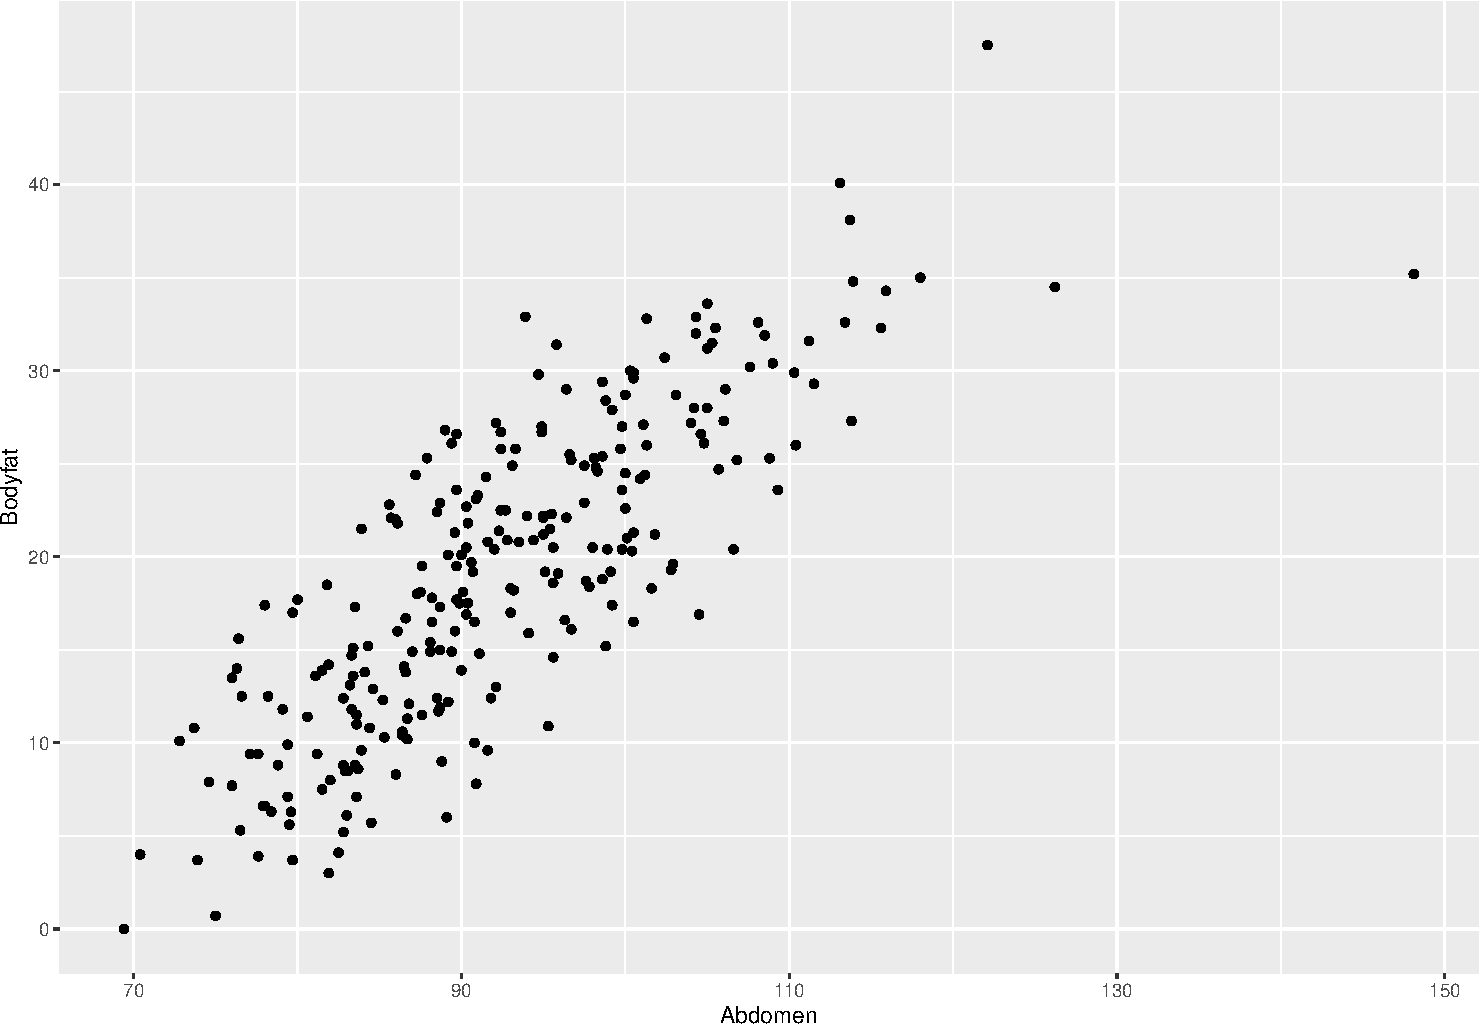
\includegraphics[width=0.9\linewidth]{Part1_intro_files/figure-beamer/unnamed-chunk-2-1} \end{center}
\end{frame}

\begin{frame}{Build a Bayesian model, a simple example}
\protect\hypertarget{build-a-bayesian-model-a-simple-example-1}{}
\begin{enumerate}
\setcounter{enumi}{1}
\tightlist
\item
  We formulate questions ..
\end{enumerate}

\begin{center}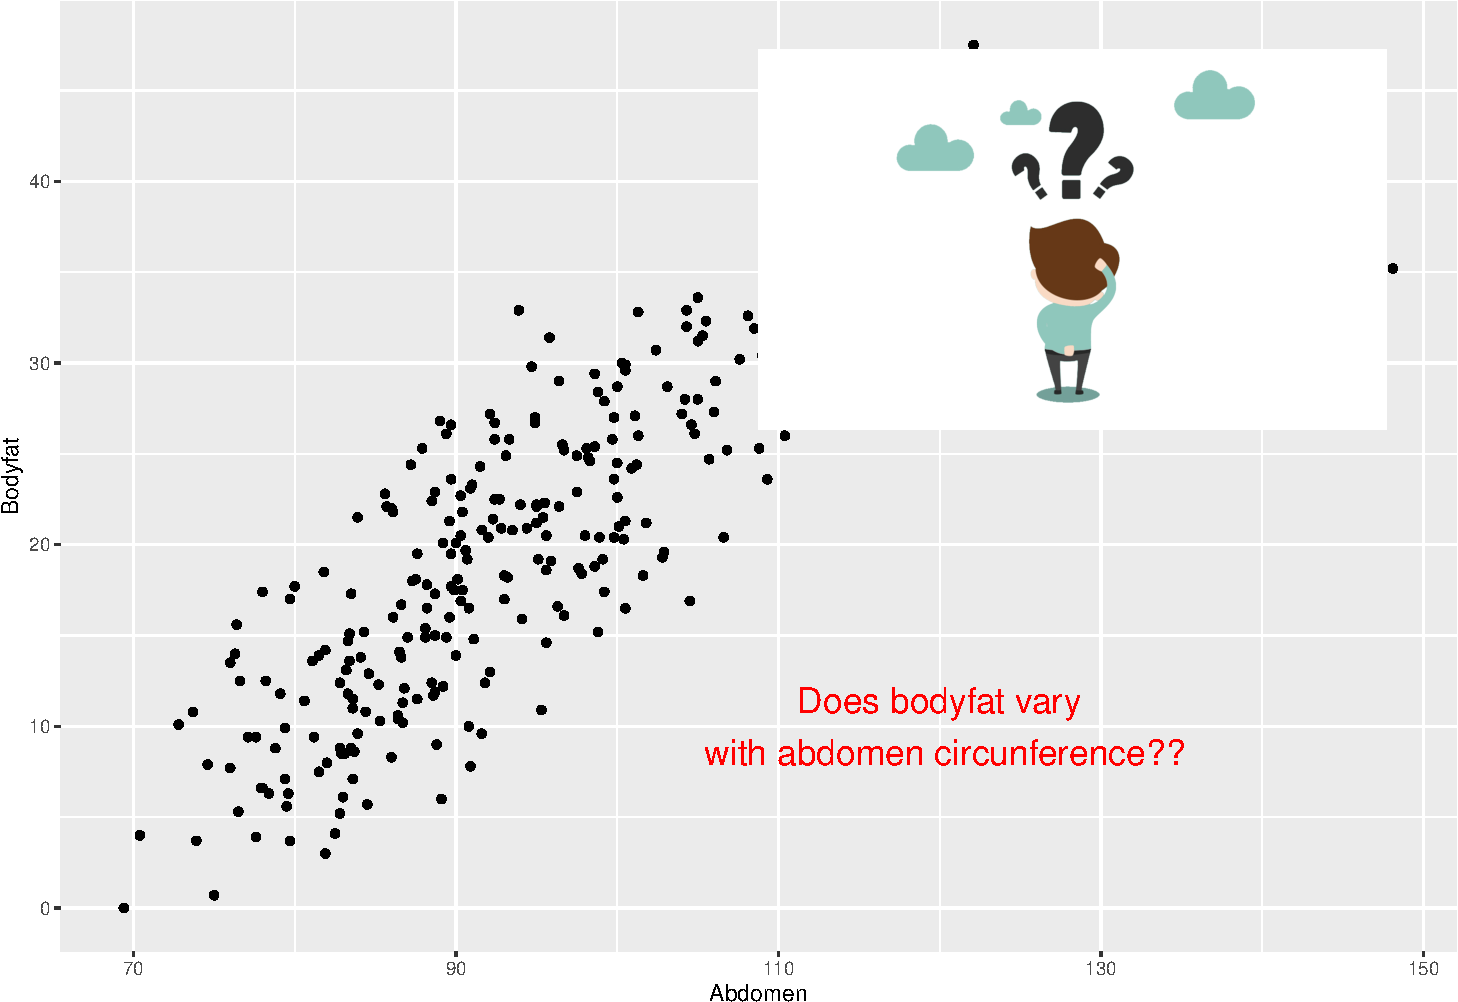
\includegraphics[width=0.6\linewidth]{Part1_intro_files/figure-beamer/unnamed-chunk-3-1} \end{center}
\end{frame}

\begin{frame}{Build a Bayesian model, a simple example}
\protect\hypertarget{build-a-bayesian-model-a-simple-example-2}{}
\begin{enumerate}
\setcounter{enumi}{2}
\tightlist
\item
  We formulate a model to answer the questions ..
\end{enumerate}

\begin{itemize}
\tightlist
\item
  The observational model
\item
  How data depend on each other/ or other quantities
\item
  What is our ``information'' prior to the observation process
\end{itemize}
\end{frame}

\begin{frame}{A Bayesian regression model}
\protect\hypertarget{a-bayesian-regression-model}{}
\begin{itemize}
\tightlist
\item
  Perc. Body fat \((y_1, \dots, y_n)\) are Gaussian distributed

  \begin{itemize}
  \tightlist
  \item
    The mean \(\eta_i\) depends on the abdomen circunference
  \item
    The precision is constant
  \end{itemize}
\end{itemize}

\[
\begin{aligned}
  y_i|\eta_i,\tau &\sim \mathcal{N}(\eta_i,\tau^{-1})\\
  \eta_i & =  \alpha + \beta x_i
\end{aligned}
\]

\begin{itemize}
\item
  Need priors for \(\alpha\), \(\beta\), \(\tau\)

  \begin{itemize}
  \item
    \((\alpha, \beta)\sim\mathcal{N}(0, \text{diag}(\sigma^2_{\alpha}, \sigma^2_{\beta}))\)
    with \(\sigma^2_{\alpha}, \sigma^2_{\beta}\) known
  \item
    \(\tau\sim\text{Gamma}(a,b)\) with \(a,b\) known
  \end{itemize}
\end{itemize}
\end{frame}

\begin{frame}{A Bayesian hyerarchical model}
\protect\hypertarget{a-bayesian-hyerarchical-model}{}
\begin{itemize}
\tightlist
\item
  \textbf{Observation model}
\end{itemize}

\[
\mathbf{y} \mid \underbrace{\alpha,
            \beta}_{\mathbf{x}}, \underbrace{\tau}_{\mathbf{\theta}}
\] Encodes information about observed data

\begin{itemize}
\tightlist
\item
  \textbf{Latent model}
\end{itemize}

\[
\mathbf{x} = (\alpha, \beta, \eta)\sim\mathcal{N}(0, \mathbf{Q}^{-1}(\theta))
\]

The unobserved process

\begin{itemize}
\tightlist
\item
  \textbf{Hyperparameters } \(\theta = \tau\)
\end{itemize}
\end{frame}

\begin{frame}{Precision Matrix \(\mathbf{Q}(\theta)\)}
\protect\hypertarget{precision-matrix-mathbfqtheta}{}
\begin{center}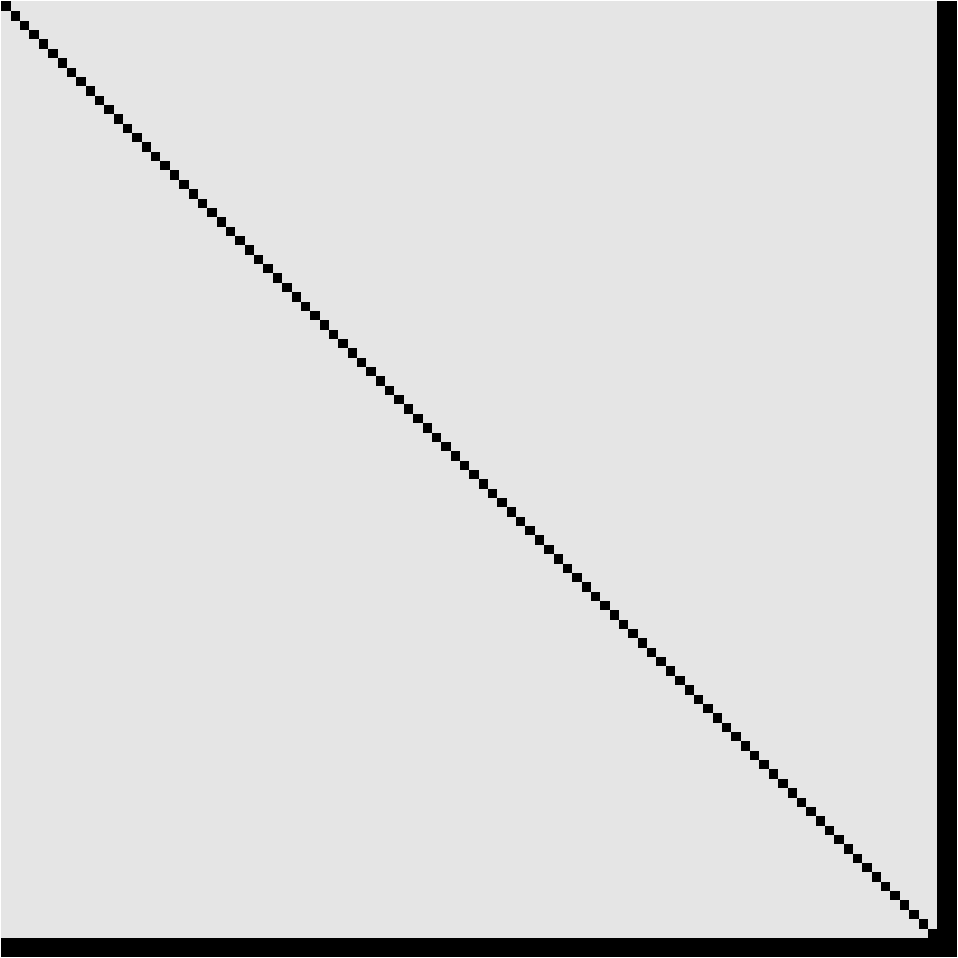
\includegraphics[width=0.6\linewidth]{Part1_intro_files/figure-beamer/unnamed-chunk-5-1} \end{center}
\end{frame}

\begin{frame}{Bayesian Computations}
\protect\hypertarget{bayesian-computations}{}
From this we can compute the \textcolor{red}{posterior distribution} \[
\pi(\mathbf{x}, \theta | \mathbf{y}) \propto \pi(\mathbf{y} | \mathbf{x},
     \theta) \pi(\mathbf{x}) \pi(\theta)
\] and then the corresponding
\textcolor{red}{posterior marginal distributions}: \[
\begin{aligned}
  \pi(x_j|\mathbf{y}) &\qquad  j = 1,2\\
  \pi(\tau|\mathbf{y})& \\
  \pi(\eta_i|\mathbf{y}) &\qquad  i = 1,\dots,n
\end{aligned}
\]
\end{frame}

\begin{frame}{Results}
\protect\hypertarget{results}{}
\begin{itemize}
\tightlist
\item
  Assign priors to \(\alpha,\beta,\tau\)
\item
  Use Bayes theorem to compute posterior distributions
\end{itemize}

\begin{center}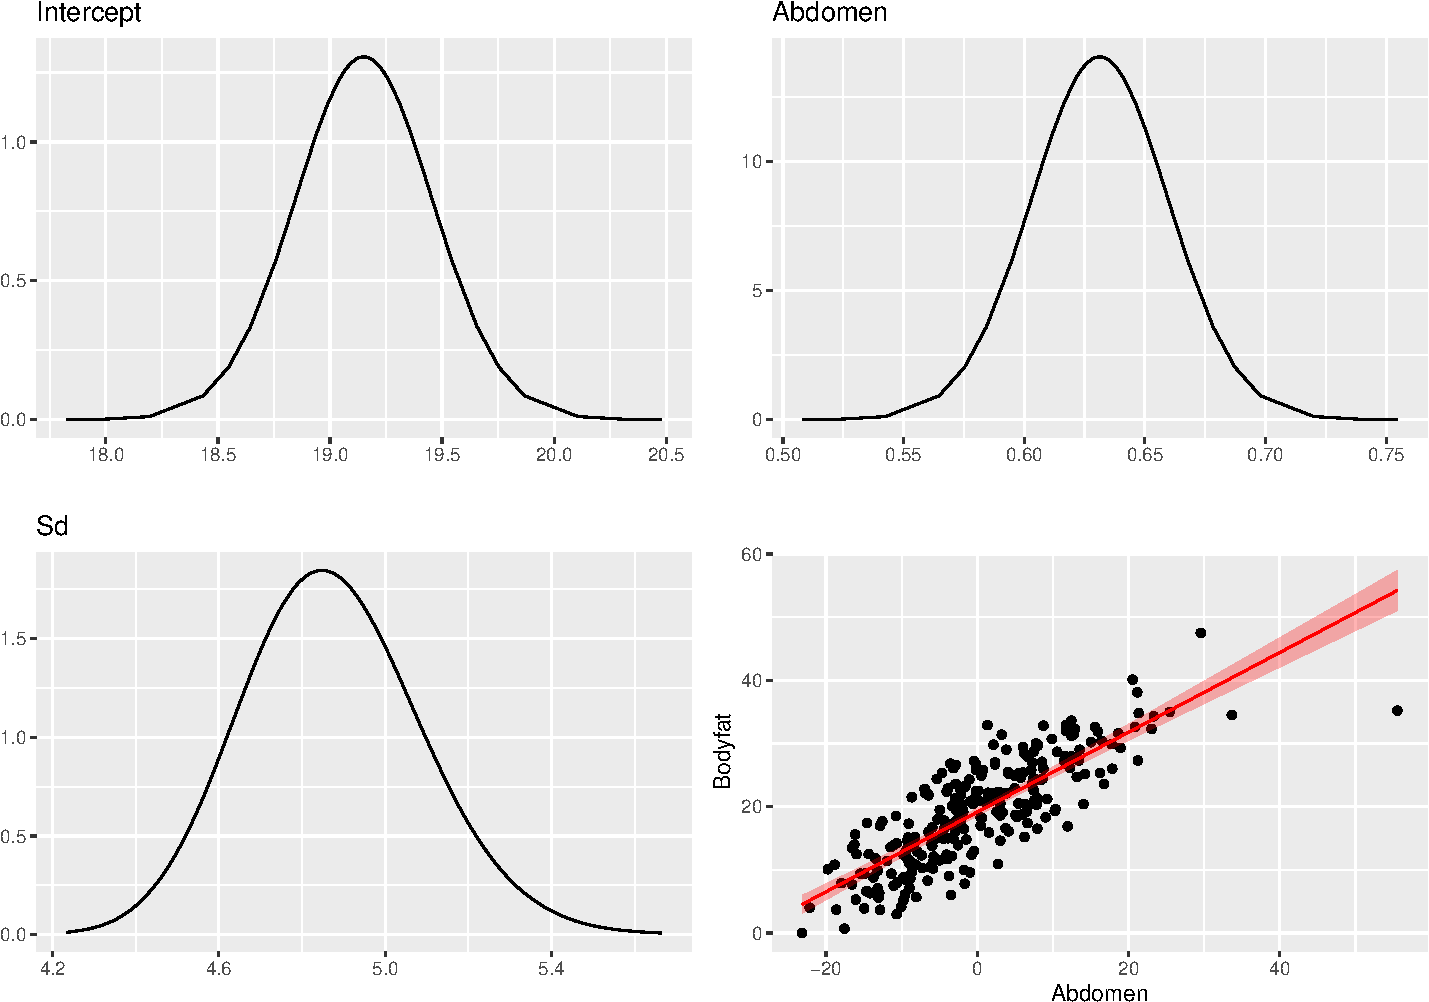
\includegraphics[width=0.6\linewidth]{Part1_intro_files/figure-beamer/unnamed-chunk-7-1} \end{center}
\end{frame}

\begin{frame}{On the prior choice\ldots.}
\protect\hypertarget{on-the-prior-choice.}{}
\begin{itemize}
\tightlist
\item
  Priors are an important part of the model
\item
  There are several ``schools'' about priors
\item
  ``non-informative'' priors are not always a good choice
\item
  for complex models priors can have a large influence on the results.
\end{itemize}
\end{frame}

\begin{frame}{Real-world datasets are usually much more complicated!}
\protect\hypertarget{real-world-datasets-are-usually-much-more-complicated}{}
Using a Bayesian framework:

\begin{itemize}
\tightlist
\item
  Build (hierarchical) models to account for potentially complicated
  dependency structures in the data.
\item
  Attribute uncertainty to model parameters and latent variables using
  priors.
\end{itemize}

\textbf{Two main challenges:}

\begin{enumerate}
\tightlist
\item
  Need computationally efficient methods to calculate posteriors.
\item
  Select priors in a sensible way
\end{enumerate}
\end{frame}

\begin{frame}{Bayesian hierarchical models}
\protect\hypertarget{bayesian-hierarchical-models-1}{}
INLA can be used with Bayesian hierarchical models where we model in
different stages or levels:

\begin{itemize}
\tightlist
\item
  \textbf{Stage 1:} What is the distribution of the responses?\\
  \strut \\
\item
  \textbf{Stage 2:} What is the distribution of the underlying
  unobserved (latent) components?\\
  \strut \\
\item
  \textbf{Stage 3:} What are our prior beliefs about the parameters
  controlling the components in the model?
\end{itemize}
\end{frame}

\begin{frame}{Stage 1: The data generating process}
\protect\hypertarget{stage-1-the-data-generating-process}{}
How is our \textcolor{red}{data (\(\boldsymbol{y}\))} generated from the
\textcolor{red}{underlying components  (\(\boldsymbol{x}\))} and
\textcolor{red}{hyperparameters (\(\boldsymbol{\theta}\))} in the model:

\begin{itemize}[<+->]
\tightlist
\item
  Gaussian response? (temperature, rainfall, fish weight \ldots)
\item
  Count data? (people infected with a disease in each area)
\item
  Point pattern? (locations of trees in a forest)
\item
  Binary data? (yes/no response, binary image)
\item
  Survival data? (recovery time, time to death)
\end{itemize}

\pause

This information is placed into our
\textcolor{red}{\textcolor{red}{likelihood}
    \(\pi(\boldsymbol{y} | \boldsymbol{x}, \boldsymbol{\theta})\)}
\end{frame}

\begin{frame}{Stage 1: The data generating process}
\protect\hypertarget{stage-1-the-data-generating-process-1}{}
We assume that \emph{given} the
\textcolor{red}{underlying components    (\(\boldsymbol{x}\))} and
\textcolor{red}{hyperparameters (\(\boldsymbol{\theta}\))} the data are
independent on each other

\[
\pi(\mathbf{y}|\mathbf{x},\theta) = \prod_{i\in\cal{I}}\pi(y_i|x_{i},\theta)
\] \pause

\textcolor{blue}{This implies that all the dependence structure in the data is explained in Stage II !!}

\pause

Can you think of a model that does not respect this condition?
\end{frame}

\begin{frame}{Stage 2: The dependence structure}
\protect\hypertarget{stage-2-the-dependence-structure}{}
The underlying \textcolor{red}{unobserved components \(\boldsymbol{x}\)}
are called \textcolor{red}{\bf{latent} components} and can be:

\begin{itemize}
\tightlist
\item
  Fixed effects for covariates
\item
  Unstructured random effects (individual effects, group effects)
\item
  Structured random effects (AR(1), regional effects, \ldots)
\end{itemize}

These are linked to the responses in the likelihood through linear
predictors.
\end{frame}

\begin{frame}{Stage 3: The hyperparameters}
\protect\hypertarget{stage-3-the-hyperparameters}{}
The likelihood and the latent model typically have hyperparameters that
control their behavior.

The \textcolor{red}{hyperparameters \(\boldsymbol{\theta}\)} can
include:

\pause

\textcolor{red}{Examples likelihood:}

\begin{itemize}
\tightlist
\item
  Variance of observation noise
\item
  Dispersion parameter in the negative binomial model
\item
  Probability of a zero (zero-inflated models)
\end{itemize}

\pause

\textcolor{red}{Examples latent model:}

\begin{itemize}
\tightlist
\item
  Variance of unstructured effects
\item
  Correlation of multivariate effects
\item
  Range and variance of spatial effects
\item
  Autocorrelation parameter
\end{itemize}
\end{frame}

\begin{frame}{Example 1: Tokyo rainfall data}
\protect\hypertarget{example-1-tokyo-rainfall-data}{}
Rainfall over 1 mm in the Tokyo area for each calendar day during two
years (1983-84) are registered.

\begin{center}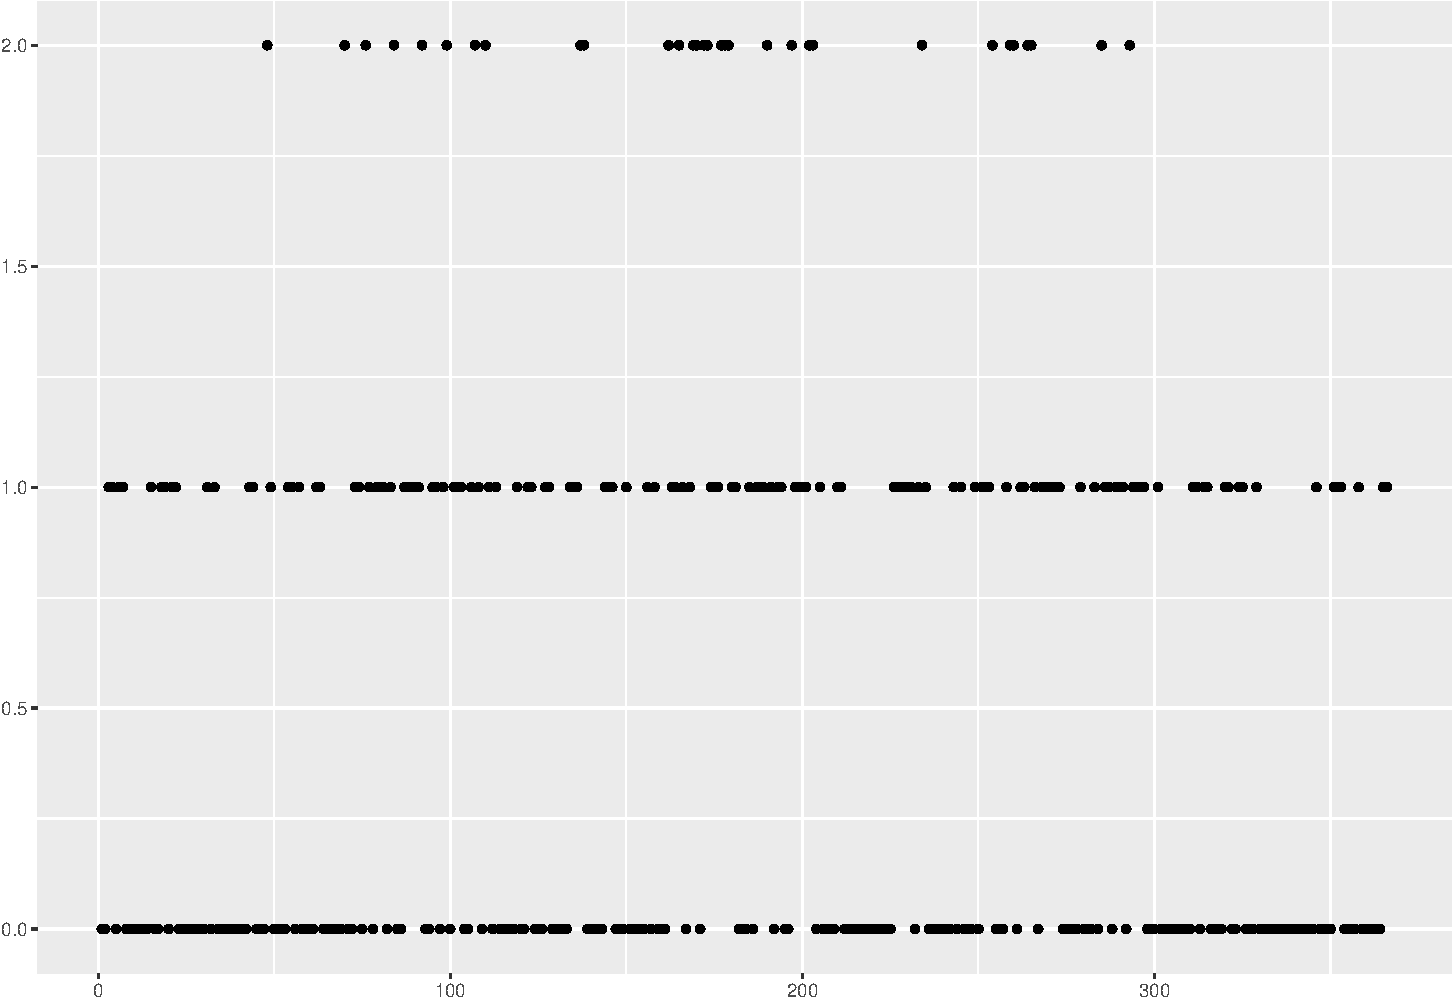
\includegraphics[width=0.6\linewidth]{Part1_intro_files/figure-beamer/unnamed-chunk-8-1} \end{center}
\end{frame}

\begin{frame}{Tokyo rainfall data}
\protect\hypertarget{tokyo-rainfall-data}{}
Rainfall over 1 mm in the Tokyo area for each calendar day during two
years (1983-84) are registered.

\begin{center}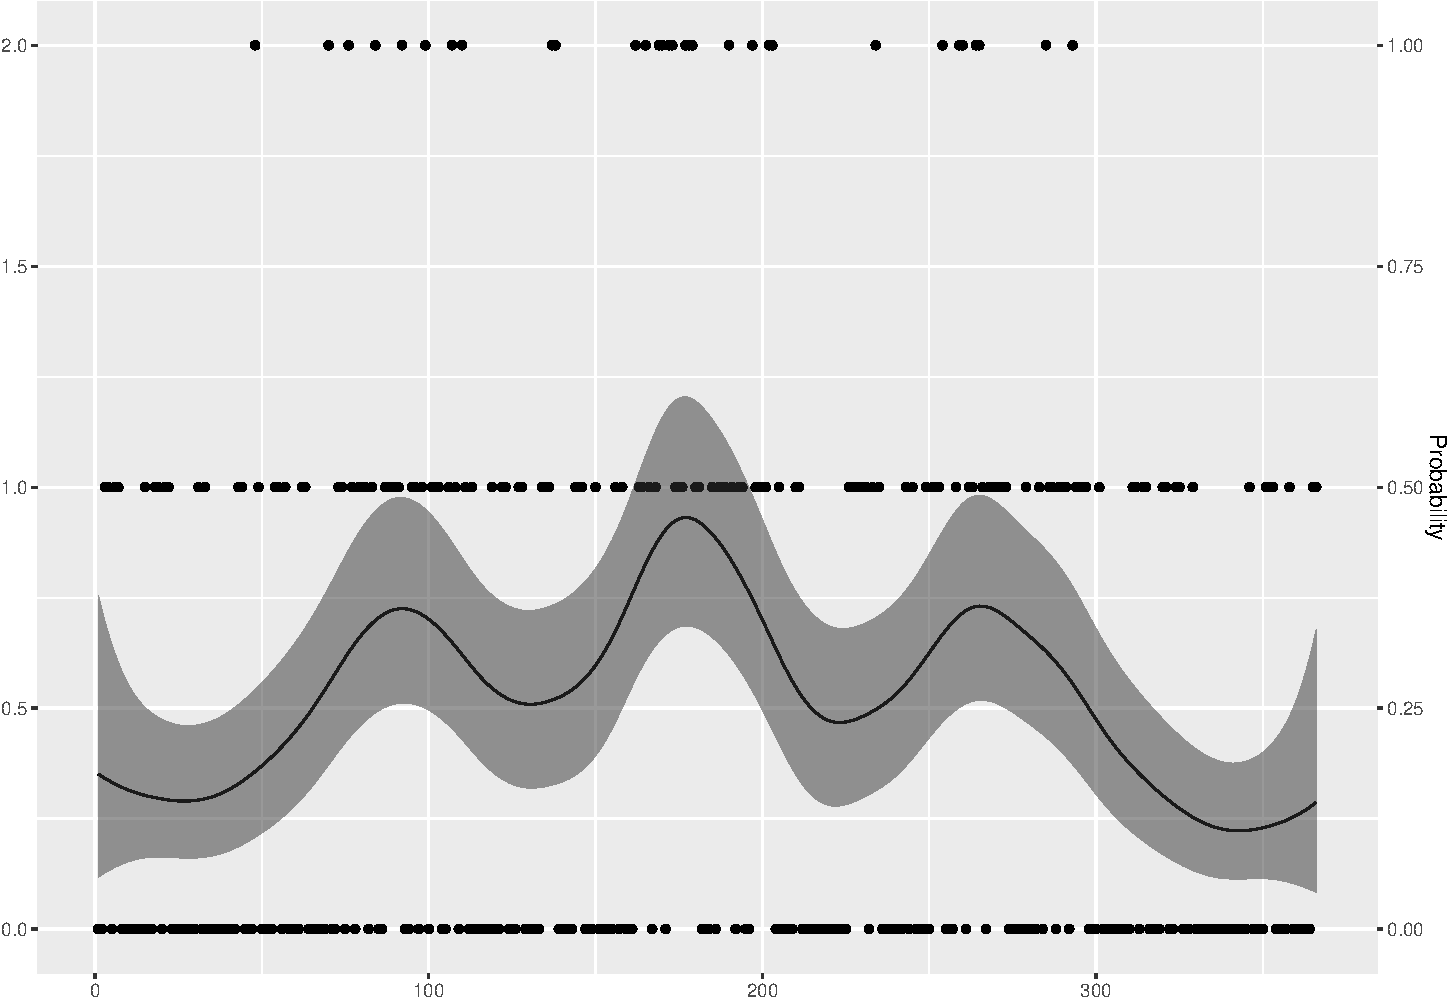
\includegraphics[width=0.6\linewidth]{Part1_intro_files/figure-beamer/unnamed-chunk-9-1} \end{center}
\end{frame}

\begin{frame}{Stage 1: The data}
\protect\hypertarget{stage-1-the-data}{}
\textcolor{red}{
$$
y_i\mid p_i \sim \text{Binomial}(n_i, p_i),
$$} for \(i=1,2,...,366\)

\[
n_{i} = \left\{
 \begin{array}{lr}
1, & \text{for}\; 29\; \text{February}\\
2, & \text{other days}
\end{array}\right.
\] \[
y_{i} =
\begin{cases}
\{0,1\}, & \text{for}\; 29\; \text{February}\\
\{0,1,2\}, & \text{other days}
 \end{cases}
\]

Linear predictor \[
logit(p_i) = \eta_i \quad \Leftrightarrow \quad p_i = \frac{1}{1+\exp(-\eta_i)}
\]

\begin{itemize}
\tightlist
\item
  probability of rain on day \(i\) depends on \(\eta_i\)
\item
  the likelihood has no hyperparameters \(\theta\)
\end{itemize}
\end{frame}

\begin{frame}{Stage 2: The latent model}
\protect\hypertarget{stage-2-the-latent-model}{}
\[
\eta_i = \alpha +  u_i + v_i
\] where

\begin{itemize}[<+->]
\tightlist
\item
  \(\alpha\) is a global mean (Gaussian)
\end{itemize}

\begin{itemize}[<+->]
\tightlist
\item
  \(\mathbf{u}\) is a AR-model like \[
  u_i  = \phi u_{i-1} + \epsilon_i, \qquad \epsilon_i\sim\mathcal{N}(0, \sigma^2_{\epsilon})
  \] with parameters \((\phi, \sigma_{\epsilon})\)
\end{itemize}

\begin{itemize}[<+->]
\tightlist
\item
  \(\mathbf{v}\) can be a unstructured term/``random effect''/slowly
  varying trend. Typically Gaussian with precision parameter \(\tau_v\)
  controlling the smoothness.
\end{itemize}

\pause

This gives the latent model
\(\mathbf{x} = (\alpha, \mathbf{u}, \mathbf{v}, \mathbf{\eta})\sim\mathcal{N}(0, \mathbf{Q}^{-1}(\theta))\).
\end{frame}

\begin{frame}{Stage 3: Hyperparameters}
\protect\hypertarget{stage-3-hyperparameters}{}
Hyperparameters control the smoothness of the effects in the latent
model

\[
\theta = (\phi, \sigma_{\epsilon}, \sigma_v)
\]
\end{frame}

\begin{frame}{The model}
\protect\hypertarget{the-model}{}
We can write the model as

\[
\begin{aligned}
\theta & \sim \pi(\theta)\\
\mathbf{x}|\theta& \sim \pi(\mathbf{x}|\theta)\\
\mathbf{y}|\mathbf{x},\theta & \sim \prod_i\pi(y_i|\eta_i,\theta)
\end{aligned}
\]
\end{frame}

\begin{frame}{Precision matrix}
\protect\hypertarget{precision-matrix}{}
\begin{center}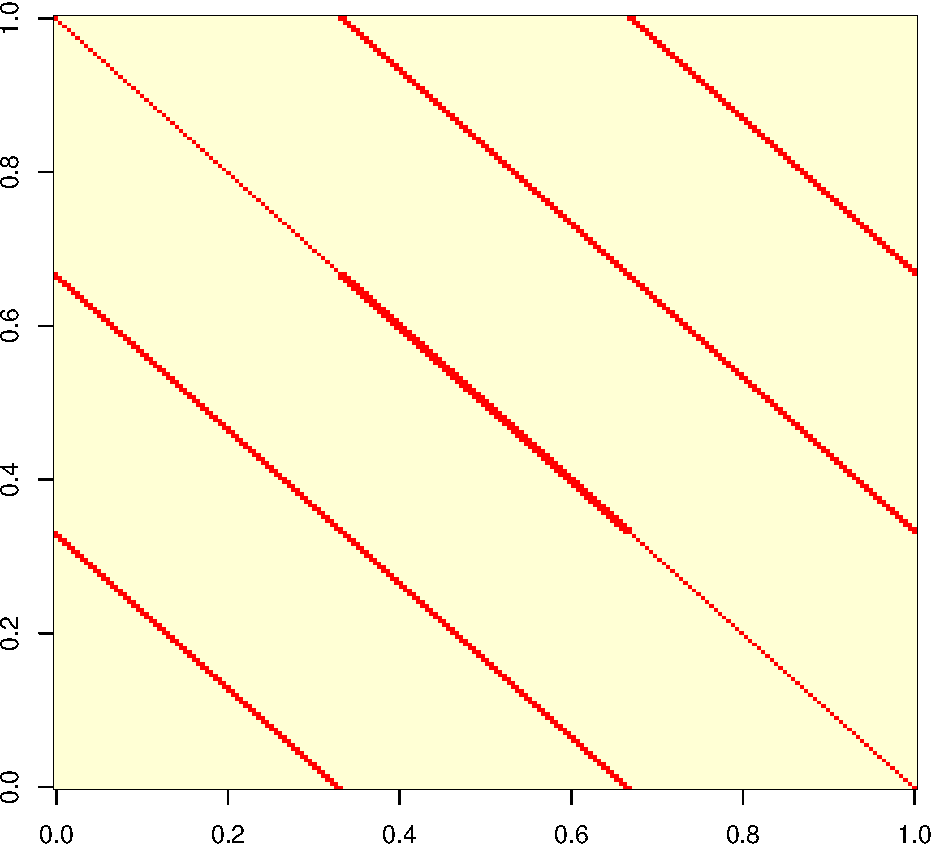
\includegraphics[width=0.8\linewidth]{graphics/Q2} \end{center}
\end{frame}

\begin{frame}{Example: disease mapping}
\protect\hypertarget{example-disease-mapping}{}
We observed larynx cancer mortality counts for males in 544 district of
Germany from 1986 to 1990 and want to understand the spatial
distribution and the inpact of covariates.

\begin{cols}

\begin{col}{0.55\textwidth}

\begin{itemize}
\tightlist
\item
  \(y_i\): The count at location \(i\).
\item
  \(E_i\): An offset; expected number of cases in district \(i\).
\item
  \(c_i\): A covariate (level of smoking consumption) at \(i\)
\item
  \(\boldsymbol{s}_i\): spatial location \(i\) .
\end{itemize}

\end{col}

\begin{col}{0.05\textwidth}

\end{col}

\begin{col}{0.4\textwidth}

\begin{center}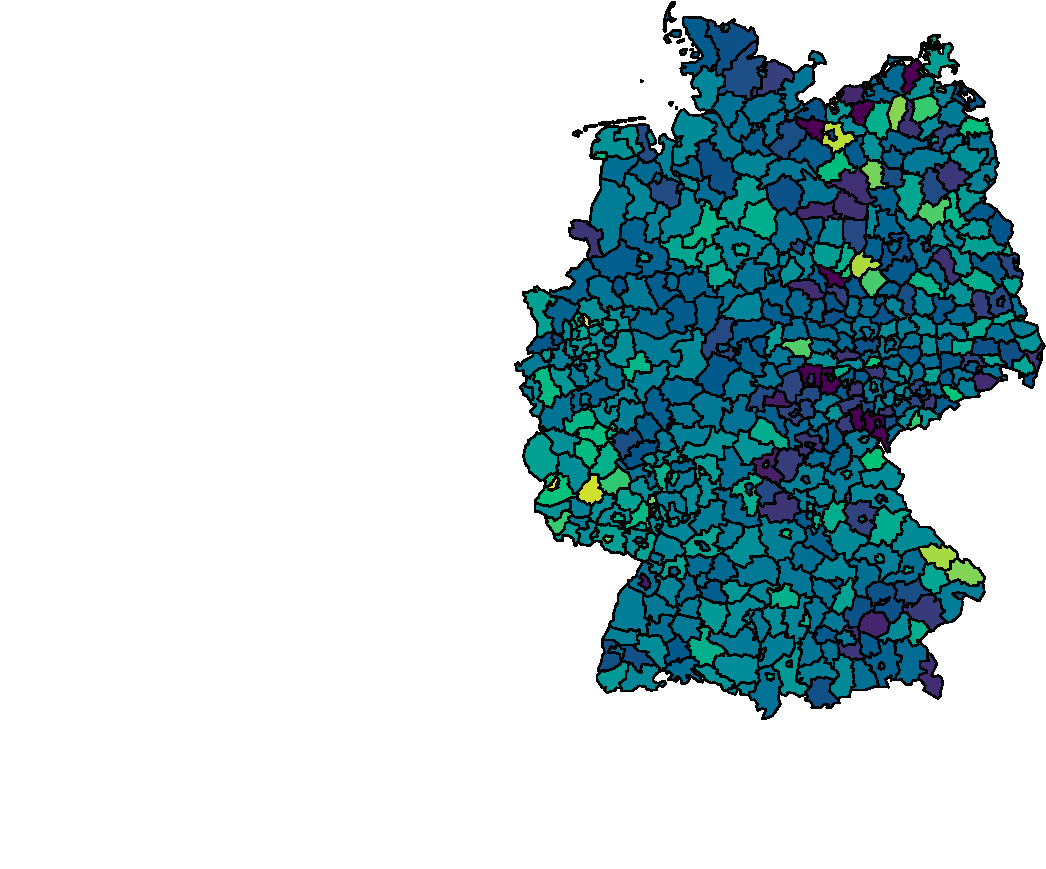
\includegraphics[width=1.1\linewidth]{Part1_intro_files/figure-beamer/unnamed-chunk-11-1} \end{center}

\end{col}

\end{cols}
\end{frame}

\begin{frame}{Bayesian disease mapping}
\protect\hypertarget{bayesian-disease-mapping}{}
\begin{itemize}[<+->]
\tightlist
\item
  \textbf{Stage 1:} We choose a Poisson distribution for the responses,
  so that \[
  y_i \mid \eta_i \sim \text{Poisson}(E_i\exp(\eta_i)))
  \]
\item
  \textbf{Stage 2:} \(\eta_i\) is a linear function of the latent
  components: a covariate \(c_i\), a spatially structured effect
  \(\mathbf{u}\), an unstructured effect \(\mathbf{v}\) likelihood by \[
  \eta_i = \mu+ \beta\ c_i + u_i + v_i
  \]
\item
  \textbf{Stage 3:}

  \begin{itemize}[<+->]
  \tightlist
  \item
    \(\tau_u\): Precision parameter for the structured effect
  \item
    \(\tau_v\): Precision parameter for the unstructured effect \pause\\
  \end{itemize}
\end{itemize}

The latent field is
\textcolor{red}{$\boldsymbol{x} = (\mu, \beta,\mathbf{u},\mathbf{v})$},
the hyperparameters are
\textcolor{red}{ $\boldsymbol{\theta} = (\tau_u,\tau_v)$}, and must be
given a prior.
\end{frame}

\begin{frame}{The model}
\protect\hypertarget{the-model-1}{}
We can write the model as

\[
\begin{aligned}
\theta & \sim \pi(\theta)\\
\mathbf{x}|\theta& \sim \pi(\mathbf{x}|\theta)\\
\mathbf{y}|\mathbf{x},\theta & \sim \prod_i\pi(y_i|\eta_i,\theta)
\end{aligned}
\]

Identical as the one before!!!!
\end{frame}

\begin{frame}{Precision Matrix}
\protect\hypertarget{precision-matrix-1}{}
\begin{center}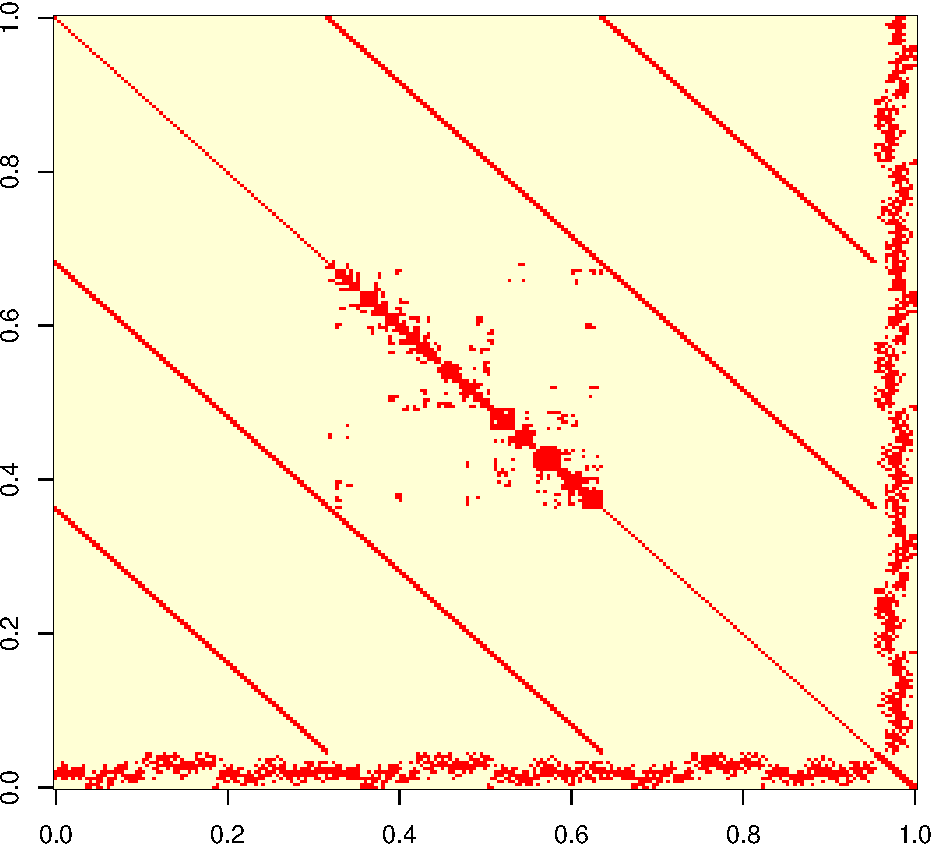
\includegraphics[width=0.8\linewidth]{graphics/Q3} \end{center}
\end{frame}

\hypertarget{latent-gaussian-models}{%
\section{Latent Gaussian models}\label{latent-gaussian-models}}

\begin{frame}{What have we learned so far}
\protect\hypertarget{what-have-we-learned-so-far}{}
Models of the kind: \[
\begin{aligned}
\theta & \sim \pi(\theta)\\
\mathbf{x}|\theta& \sim \pi(\mathbf{x}|\theta) = \mathcal{N}(0, \mathbf{Q}^{-1}(\theta))\\
\mathbf{y}|\mathbf{x},\theta & \sim \prod_i\pi(y_i|\eta_i,\theta)
\end{aligned}
\] occurs in many, seemingly unrelated, statistical models.

We call this \textcolor{red}{\bf Latent Gaussian models}.
\end{frame}

\begin{frame}{Other example of LGM}
\protect\hypertarget{other-example-of-lgm}{}
\begin{itemize}
\tightlist
\item
  Generalised linear (mixed) models
\item
  Stochastic volatility
\item
  Generalised additive (mixed) models
\item
  Measurement error models
\item
  Spline smoothing
\item
  Semiparametric regression
\item
  Space-varying (semiparametric) regression models
\item
  Disease mapping
\item
  Log-Gaussian Cox-processes
\item
  Model-based geostatistics (*)
\item
  Spatio-temporal models
\item
  Survival analysis
\item
  +++
\end{itemize}
\end{frame}

\begin{frame}{Characteristics of LGM}
\protect\hypertarget{characteristics-of-lgm}{}
\begin{itemize}
\item
  The \textcolor{red}{latent part} of the hierarchical model is
  \textcolor{red}{Gaussian}: \[
  \boldsymbol{x} | \boldsymbol{\theta} \sim N(0, {Q}^{-1}(\theta))
  \]
\item
  The expected value is \(\boldsymbol{0}\)
\item
  The \emph{precision} matrix (inverse covariance matrix) is
  \({Q}(\theta)\)
\end{itemize}
\end{frame}

\begin{frame}{The general set-up}
\protect\hypertarget{the-general-set-up}{}
The mean of the observation \(i\), \(\mu_i\), is connected to the linear
predictor, \(\eta_i\), through a link function \(g\), \[
\eta_i = g(\mu_i) = \mu + \boldsymbol{z}_i^\top \boldsymbol{\beta}+\sum_{\gamma} w_{\gamma, i} f_\gamma(c_{\gamma,i})+v_i, \quad i = 1,2,\ldots,n
\]

where \[
\begin{aligned}
\mu &: \text{Intercept}\\
        \boldsymbol{\beta} &: \text{Fixed effects of covariates \(\boldsymbol{z}\)}\\
        \{f_\gamma(\cdot)\} &: \text{Non-linear/smooth effects of covariates \(\boldsymbol{c}\)}\\
        \{w_{\gamma,i}\} &: \text{Known weights defined for each observed data point}\\
        \boldsymbol{v} &: \text{Unstructured error terms}
\end{aligned}
\]
\end{frame}

\begin{frame}{Specification of the latent field}
\protect\hypertarget{specification-of-the-latent-field}{}
\begin{itemize}[<+->]
\tightlist
\item
  Collect all parameters (random variables) in the
  \textcolor{red}{latent field}
  \(\mathbf{x} =\{\mu, {\beta}, \{f_\gamma(\cdot)\}, {\eta}\}\).
\item
  A latent Gaussian model is obtained by assigning Gaussian priors to
  all elements of \(\mathbf{x}\).
\item
  Very flexible due to many different forms of the unknown functions
  \(\{f_\gamma(\cdot)\}\):
\item
  \textcolor{red}{Hyperparameters} account for variability and
  length/strength of dependence
\end{itemize}
\end{frame}

\begin{frame}{Flexibility through \(f\)-functions}
\protect\hypertarget{flexibility-through-f-functions}{}
The functions \(\{f_\gamma\}\) in the linear predictor make it possible
to capture very different types of random effects in the same framework:

\begin{itemize}
\tightlist
\item
  \(f(\texttt{time})\):, For example, an AR(1) process, RW1 or RW2
\item
  \(f(\texttt{spatial location})\):, For example, a Matern field
\item
  \(f(\texttt{covariate})\):, For example, a RW1 or RW2 on the covariate
  values
\item
  \(f(\texttt{time}, \texttt{spatial location})\) can be a
  spatio-temporal effect
\item
  And much more
\end{itemize}
\end{frame}

\begin{frame}{Additivity}
\protect\hypertarget{additivity}{}
\begin{itemize}
\tightlist
\item
  One of the most useful features of the framework is the additivity.
\item
  Effects can easily be removed and added without difficulty.
\item
  Each component might add a new latent part and might add new
  hyperparameters, but the modelling framework and computations stay the
  same.
\end{itemize}

\pause

\textcolor{red}{OBS:} The \emph{linear} predictor needs to stay linear!!
So effects can be added but not multiplied\\

Why??
\end{frame}

\begin{frame}{A small point to think about}
\protect\hypertarget{a-small-point-to-think-about}{}
From a Bayesian point of view fixed effects and random effects are all
the same.

\begin{itemize}
\tightlist
\item
  Fixed effects are also random
\item
  They only differ in the prior we put on them
\end{itemize}
\end{frame}

\begin{frame}{So\ldots which model fit the INLA framework??}
\protect\hypertarget{sowhich-model-fit-the-inla-framework}{}
\begin{enumerate}
\tightlist
\item
  Latent \textbf{Gaussian} model
\item
  The latent field has a sparse precision matrix (Markov properties)
\item
  The data are conditionally independent given the latent field
\item
  The predictor is linear
\end{enumerate}
\end{frame}

\begin{frame}{}
\protect\hypertarget{section}{}
\small

Assume that, given \(\eta = (\eta_1,\dots,\eta_n)\) the observations
\(y = (y_1,\dots,y_n)\) are independent and Poisson distributed with
parameter \(\lambda_ i = \exp(\eta_i)\) i.e. \[
y_i|\eta_i =\text{Poisson}(\lambda_i); i = 1,\dots,n
\]\\
1. \(\eta_i=\alpha+\beta x_i+U_i\) where \[
\begin{aligned}
\alpha,\beta & \sim\mathcal{N}(0,1)\\
U_i & \sim \mathcal{N}(0,1) \text{ for } i = 1,\dots,n
\end{aligned}
\] 2. \(\eta_i=\alpha+\beta x_i+V_i\) where \[
\begin{aligned}
\alpha,\beta & \sim\mathcal{N}(0,1)\\
V_i & \sim \text{Bernoulli}(0.4) \text{ for } i = 1,\dots,n
\end{aligned}
\] 3. \(\eta_i=\alpha+\beta x_i\) where \[
\begin{aligned}
\alpha,\beta & \sim\mathcal{N}(0,1)\\
\end{aligned}
\] 4. \(\eta_i=\alpha+\beta x_i + U_iV_i\) where \[
\begin{aligned}
\alpha,\beta & \sim\mathcal{N}(0,1)\\
U_i & \sim \mathcal{N}(0,1) \text{ for } i = 1,\dots,n\\
V_i & \sim \mathcal{N}(0,1) \text{ for } i = 1,\dots,n
\end{aligned}
\] \normalsize
\end{frame}

\begin{frame}{Why precision matrix}
\protect\hypertarget{why-precision-matrix}{}
\end{frame}

\end{document}
